\section{Solution}
Here since we need to add D-Cache and I-Cache, in the existing pipline module we would have to add an 8-length array of 32-bit registers for D-Cache and the instruction is received as an input to the pipeline module.
% \\[0.2in]
% \makebox[\textwidth]{hello}
% \begin{lstlisting}
%   import numpy as np
% \end{lstlisting}
% \begin{lstlisting}[label=some-code,caption=Some Code]
%   public void here() {
%       goes().the().code()
%   }
%   \end{lstlisting}
  
% \lstset{language=Java}
% \begin{lstlisting}
%   public class void main(String args){
    
%   }
% \end{lstlisting}

% the below is the template
% \lstset{language=Verilog}
% \begin{lstlisting}
%   module alu_with_clk(
%     input A,B
%   );
%   endmodule;
% \end{lstlisting}

The complete code for the pipeline can be found in the \href{https://github.com/nnk03/PIPELINE-GROUP-13-BATCH-2021-CO-LAB-IIT-PALAKKAD}{GITHUB REPO}

The code for pipeline and testbench is in the final section of this report \ref{code_section}.
\\
The pipeline receives the instruction as a 256 bit string. The pipeline has an instruction cache which is 8-length array of registers of 32-bit instruction named \textbf{instruction\textunderscore cache}.
For the data cache, it is also an 8-length array (named \textbf{data\textunderscore
cache}) of registers which can hold 32-bit values which is declared inside the pipeline module. When \textbf{rst is 1}, all the values inside the register file resets to zero and the \textbf{instruction\textunderscore cache} inside the pipeline module will have the correct instruction in the correct addresses. And, the whenever posedge clk happens, the pipeline which is modelled as an FSM will go from \textit{STAGE 1} to \textit{STAGE 4} at each posedge clk. \textbf{Instruction Fetch} happens when the current stage is \textit{STAGE 1}.
The type of instruction (i.e. whether it is load instruction, store instruction, or R-Type instruction or I-Type instruction) is obtained from the decoder. 
The schematic for the design is shown before the section "Code for Lab 7"$^{\ref{code_section}}$ .i.e. here \ref{schematic} (The schematic is in landscape view).

\begin{itemize}
  \item When it is a load instruction, say for example \textit{lw x28, 0(x29)}, it takes the value of \textit{x29}, adds the offset 0 and stores the value in this address of the \textbf{data\textunderscore cache} to \textit{x28}.
  \item When it is a store instruction, say for example \textit{sw x28, 0(x29)}, it stores the value in the register \textit{x28} to the \textbf{data\textunderscore cache} at the address \textit{x28} added with the offset 0.
  \item When it is an R-Type instruction, say for example, \textit{add x29, x28, x28}, it takes the value of \textit{x28} and adds it with itself and writes it to the register \textit{x29}.
  \item When it is an I-Type instruction, say for example, \textit{add x29, x28, 5}, it takes the value of \textit{x28} and adds it to \textit{5} and writes it to the register \textit{x29}.

\end{itemize}

% 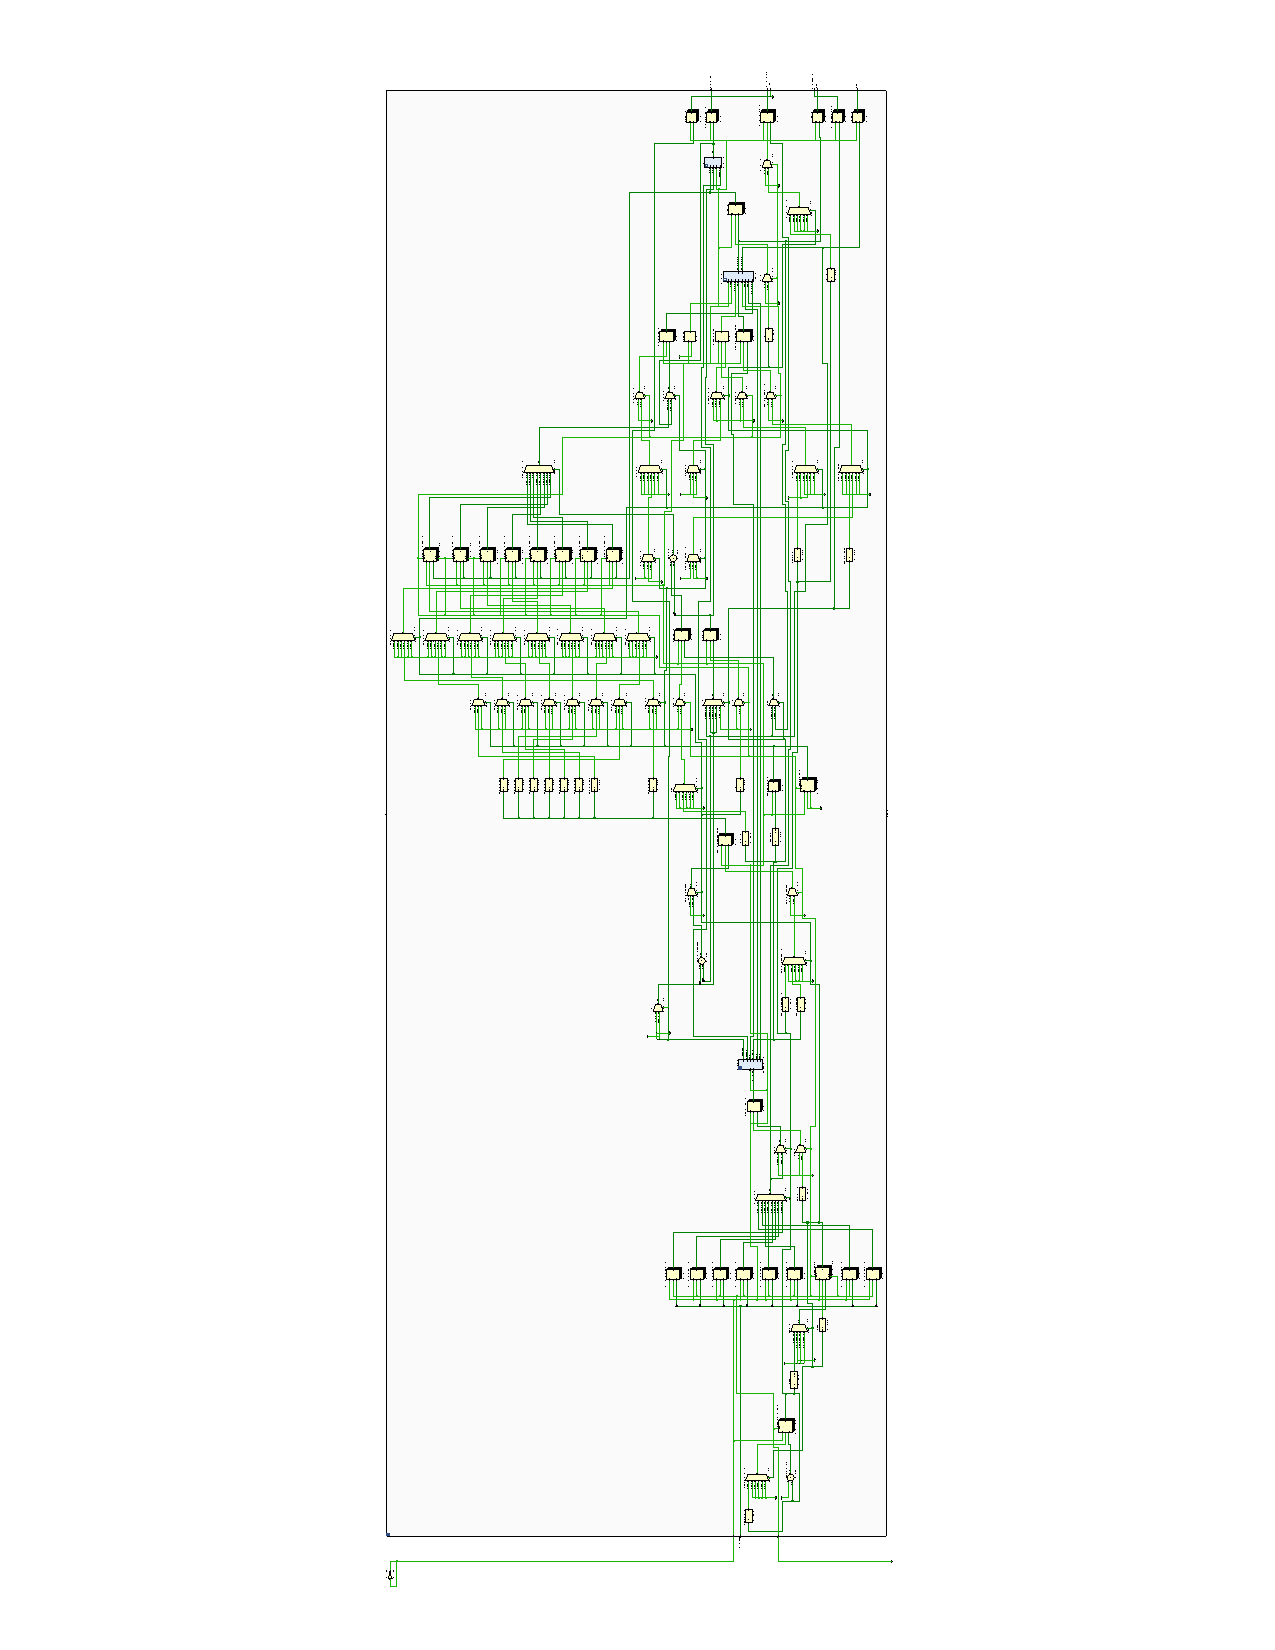
\includepdf[page={1}]{PIPELINE_LAB_7_SCHEMATIC_LANDSCAPE}

